\section{Experimentación}\label{sec:results}

\begin{frame}
    \frametitle{Clusterapp}

    \begin{itemize}
        \item<2-> Interfaz web
        \item<3-> Interfaz de línea de comandos
        \item<4-> Librería de \textit{Python}
    \end{itemize}

\end{frame}

\begin{frame}
    \frametitle{Clusterapp}

    \begin{figure}[!h]
        \centering
        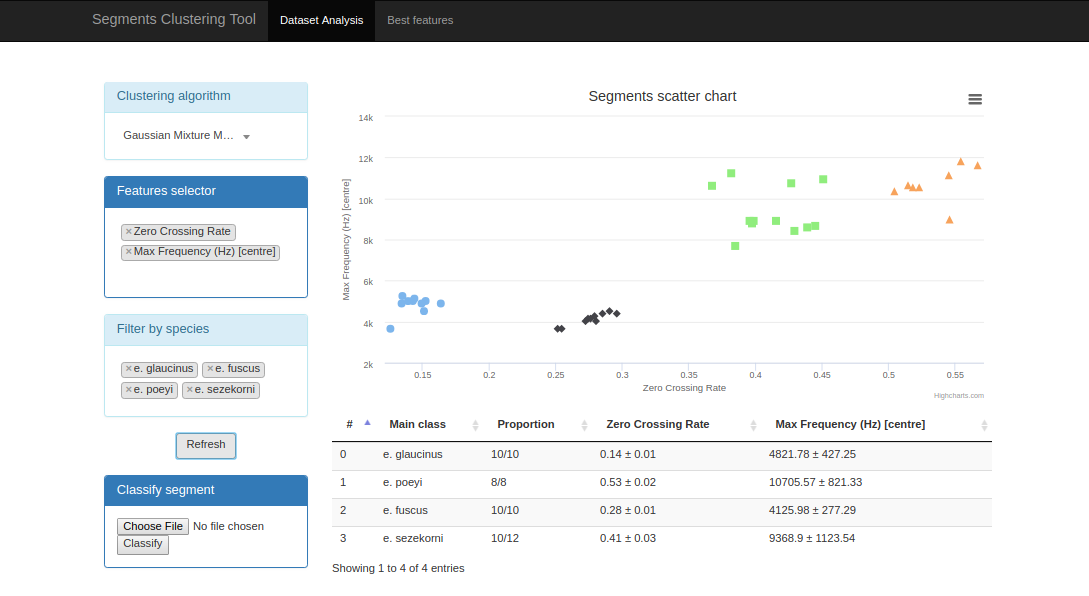
\includegraphics[width=\textwidth]{dataset-analysis.png}
    \end{figure}

\end{frame}

\begin{frame}
    \frametitle{Clusterapp}

    \begin{figure}[!h]
        \centering
        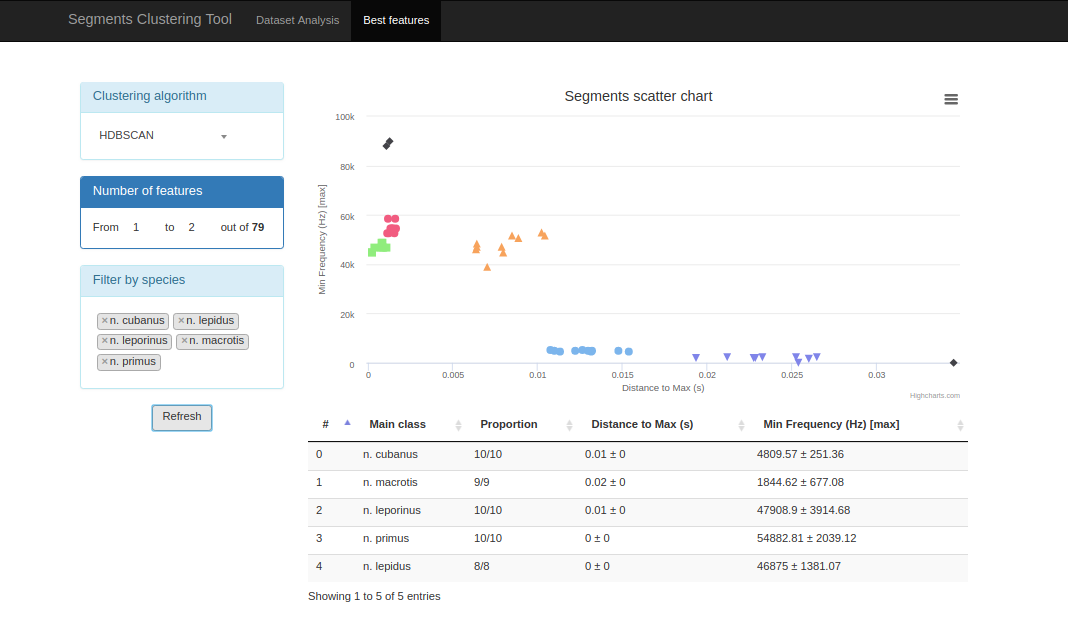
\includegraphics[width=\textwidth]{best-features.png}
    \end{figure}

\end{frame}

\begin{frame}
    \frametitle{Conjuntos de datos}

    \begin{itemize}
        \item<2-> \textit{Clases}
        \begin{itemize}
            \item<3-> Aves (230 segmentos - 23 clases - 16 especies)
            \item<4-> Insectos (184 segmentos - 10 clases - 10 especies)
        \end{itemize}
        \item<5-> \textit{Orden}
        \begin{itemize}
            \item<6-> Murciélagos (190 segmentos - 19 clases - 19 especies)
        \end{itemize}
        \item<7-> Aves + Insectos + Murciélagos (604 segmentos - 52 clases - 45 especies)
    \end{itemize}

\end{frame}

\begin{frame}
    \frametitle{Resultados}

    \begin{figure}[!h]
        \centering
        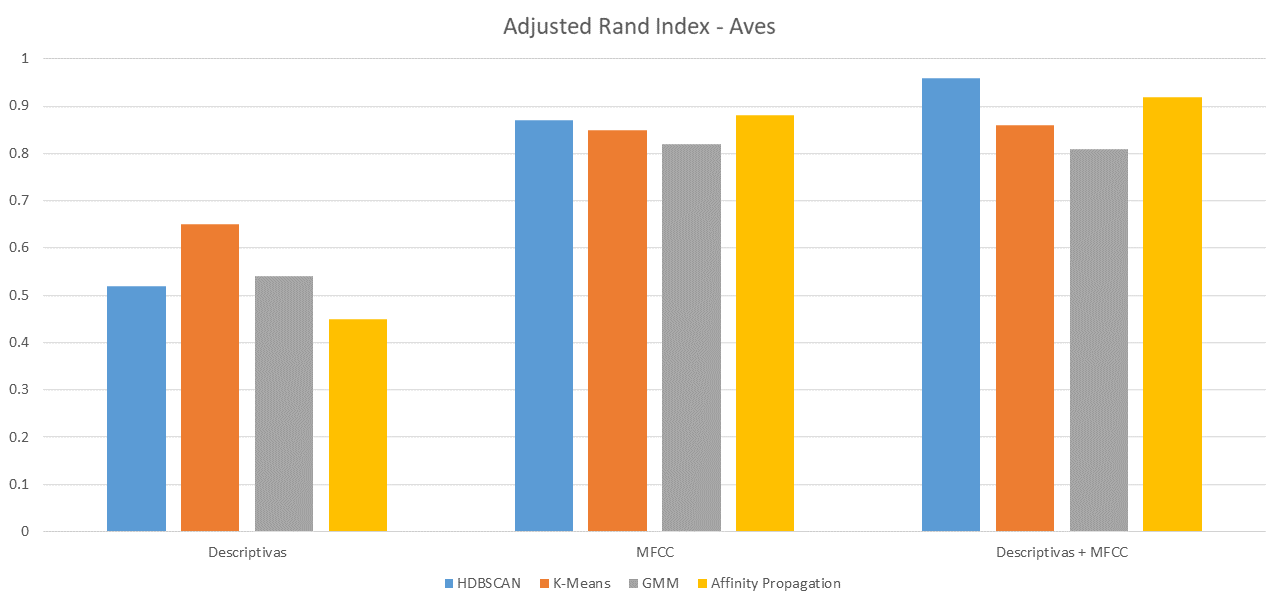
\includegraphics[width=\textwidth]{birds.png}
    \end{figure}

\end{frame}

\begin{frame}
    \frametitle{Resultados}
    \framesubtitle{Adjusted Mutual Information}

    \begin{table}[H]
        \centering
        \begin{tabular}{lllllll}
            \hline
            Algoritmo & 1 & 2 & 3 & 4 & 5 & 6  \\ \hline
            HDBSCAN & 0.71 & 0.92 & 0.96 & 0.92 & 0.91 & 0.80 \\
            K-Means & 0.79 & 0.91 & 0.92 & 0.95 & \cellcolor[HTML]{FFFC9E}0.99 & 0.83 \\
            GMM & 0.72 & 0.90 & 0.90 & 0.92 & 0.95 & 0.83 \\
            Affinity Propagation & 0.65 & 0.92 & 0.95 & 0.95 & 0.95 & 0.62
        \end{tabular}
    \end{table}

    {\tiny
    \begin{enumerate}
        \item LAT, AP, TC, ED, AC, ZCR, Frecuencia pico, Frecuencia máxima, Frecuencia mínima, Bandwidth, SC, SRO y SFX\@. %114578
        \item MFCC\@. %93
        \item LAT, AP, TC, ED, AC, ZCR, Frecuencia pico, Frecuencia máxima, Frecuencia mínima, Bandwidth, SC, SRO, SFX y MFCC\@.
        \item LAT, ZCR, Frecuencia máxima, Bandwidth, SC, SFX y MFCC\@. %57080
        \item LAT, TC, Frecuencia mínima, SFX y MFCC\@. %12910
        \item ED, ZCR y Frecuencia mínima.
        %2210
    \end{enumerate}
    }

\end{frame}

\begin{frame}
    \frametitle{Resultados}

    \begin{figure}[!h]
        \centering
        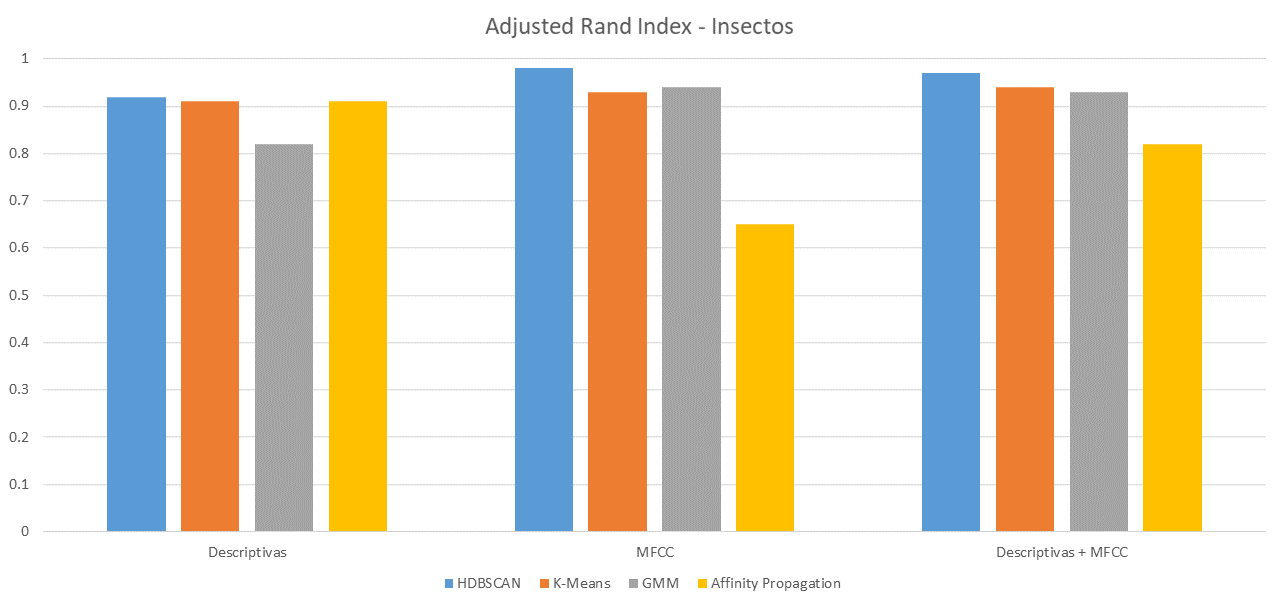
\includegraphics[width=\textwidth]{insects.png}
    \end{figure}

\end{frame}

\begin{frame}
    \frametitle{Resultados}
    \framesubtitle{Adjusted Mutual Information}

    \begin{table}[H]
        \centering
        \begin{tabular}{lllllll}
            \hline
            Algoritmo & 1 & 2 & 3 & 4 & 5 & 6  \\ \hline
            HDBSCAN & 0.93 & 0.97 & 0.96 & 0.96 & 0.97 & 0.79 \\
            K-Means & 0.94 & 0.95 & 0.96 & 0.95 & 0.96 & 0.95 \\
            GMM & 0.87 & 0.96 & 0.95 & 0.95 & 0.96 & \cellcolor[HTML]{FFFC9E}0.98 \\
            Affinity Propagation & 0.93 & 0.82 & 0.71 & 0.86 & 0.71 & 0.81
        \end{tabular}
    \end{table}

    {\tiny
    \begin{enumerate}
        \item LAT, AP, TC, ED, AC, ZCR, Frecuencia pico, Frecuencia máxima, Frecuencia mínima, Bandwidth, SC, SRO y SFX\@. %114578
        \item MFCC\@. %93
        \item LAT, AP, TC, ED, AC, ZCR, Frecuencia pico, Frecuencia máxima, Frecuencia mínima, Bandwidth, SC, SRO, SFX y MFCC\@.
        \item LAT, ZCR, Frecuencia máxima, Bandwidth, SC, SFX y MFCC\@. %57080
        \item LAT, TC, Frecuencia mínima, SFX y MFCC\@. %12910
        \item ED, ZCR y Frecuencia mínima.
        %2210
    \end{enumerate}
    }

\end{frame}

\begin{frame}
    \frametitle{Resultados}

    \begin{figure}[!h]
        \centering
        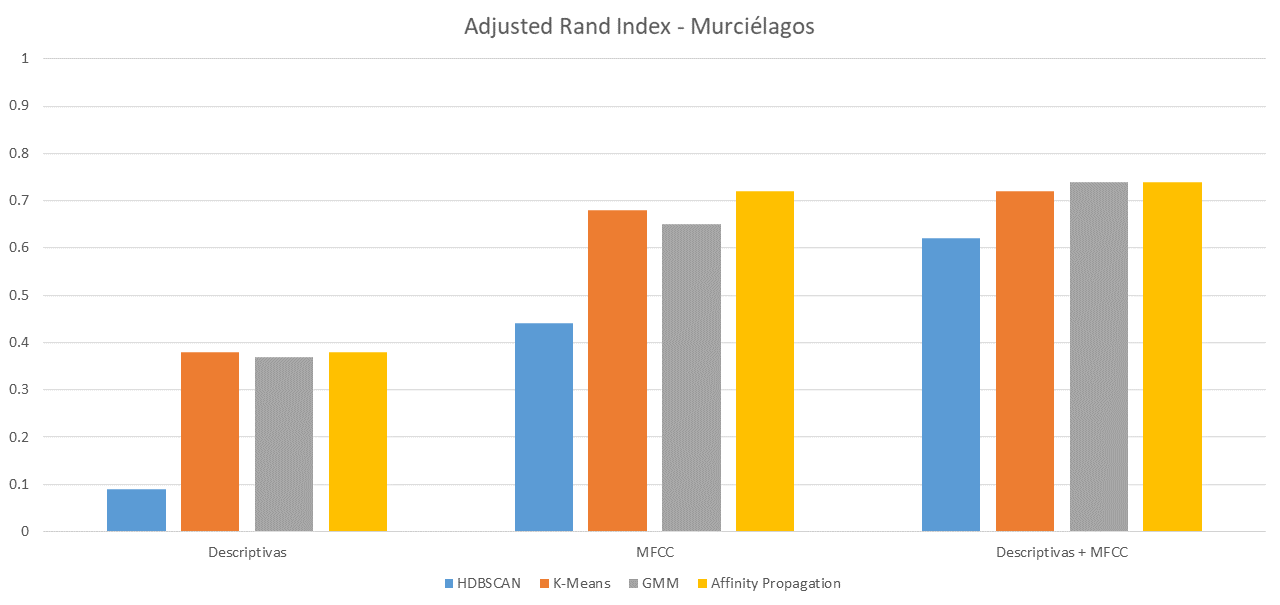
\includegraphics[width=\textwidth]{bats.png}
    \end{figure}

\end{frame}

\begin{frame}
    \frametitle{Resultados}
    \framesubtitle{Adjusted Mutual Information}

    \begin{table}[H]
        \centering
        \begin{tabular}{lllllll}
            \hline
            Algoritmo & 1 & 2 & 3 & 4 & 5 & 6  \\ \hline
            HDBSCAN & 0.26 & 0.67 & 0.75 & 0.73 & 0.67 & 0.52 \\
            K-Means & 0.59 & 0.80 & 0.82 & \cellcolor[HTML]{FFFC9E}0.91 & 0.81 & 0.67 \\
            GMM & 0.57 & 0.78 & 0.84 & 0.83 & 0.79 & 0.66 \\
            Affinity Propagation & 0.57 & 0.81 & 0.85 & 0.87 & 0.85 & 0.57
        \end{tabular}
    \end{table}

    {\tiny
    \begin{enumerate}
        \item LAT, AP, TC, ED, AC, ZCR, Frecuencia pico, Frecuencia máxima, Frecuencia mínima, Bandwidth, SC, SRO y SFX\@. %114578
        \item MFCC\@. %93
        \item LAT, AP, TC, ED, AC, ZCR, Frecuencia pico, Frecuencia máxima, Frecuencia mínima, Bandwidth, SC, SRO, SFX y MFCC\@.
        \item LAT, ZCR, Frecuencia máxima, Bandwidth, SC, SFX y MFCC\@. %57080
        \item LAT, TC, Frecuencia mínima, SFX y MFCC\@. %12910
        \item ED, ZCR y Frecuencia mínima.
        %2210
    \end{enumerate}
    }

\end{frame}

\begin{frame}
    \frametitle{Resultados}

    \begin{figure}[!h]
        \centering
        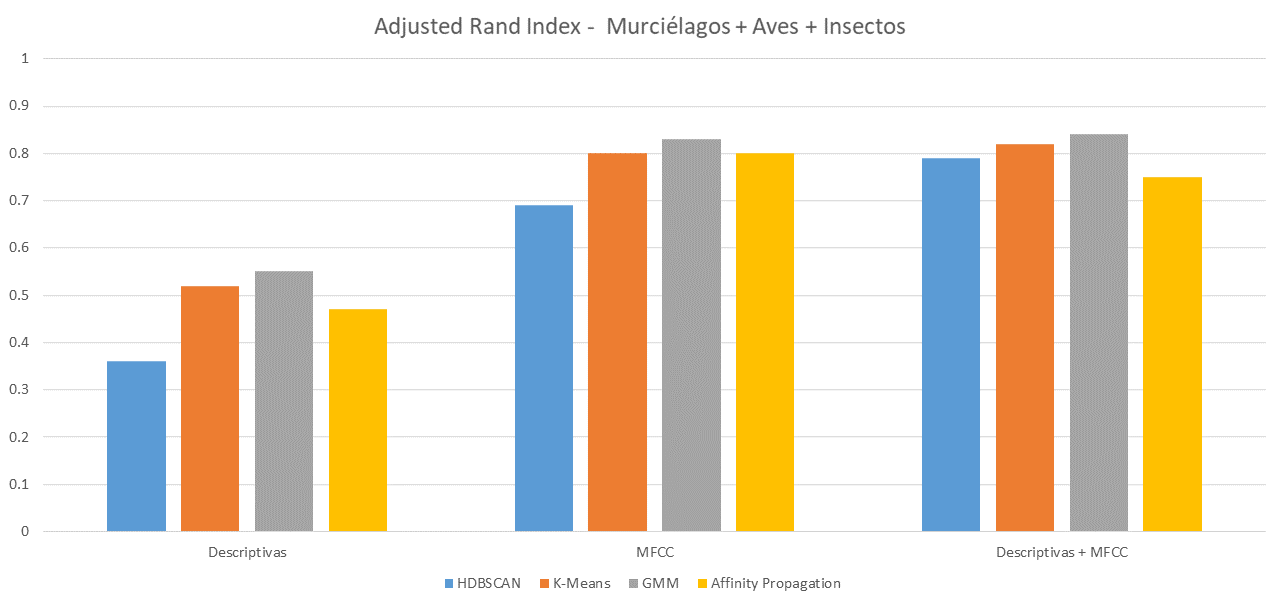
\includegraphics[width=\textwidth]{all.png}
    \end{figure}

\end{frame}

\begin{frame}
    \frametitle{Resultados}
    \framesubtitle{Adjusted Mutual Information}

    \begin{table}[H]
        \centering
        \begin{tabular}{lllllll}
            \hline
            Algoritmo & 1 & 2 & 3 & 4 & 5 & 6  \\ \hline
            HDBSCAN & 0.61 & 0.85 & 0.90 & 0.86 & 0.87 & 0.72 \\
            K-Means & 0.69 & 0.88 & 0.87 & \cellcolor[HTML]{FFFC9E}0.91 & 0.88 & 0.76 \\
            GMM & 0.70 & 0.88 & 0.90 & 0.87 & \cellcolor[HTML]{FFFC9E}0.91 & 0.77 \\
            Affinity Propagation & 0.63 & 0.89 & 0.84 & 0.87 & 0.86 & 0.56
        \end{tabular}
    \end{table}

    {\tiny
    \begin{enumerate}
        \item LAT, AP, TC, ED, AC, ZCR, Frecuencia pico, Frecuencia máxima, Frecuencia mínima, Bandwidth, SC, SRO y SFX\@. %114578
        \item MFCC\@. %93
        \item LAT, AP, TC, ED, AC, ZCR, Frecuencia pico, Frecuencia máxima, Frecuencia mínima, Bandwidth, SC, SRO, SFX y MFCC\@.
        \item LAT, ZCR, Frecuencia máxima, Bandwidth, SC, SFX y MFCC\@. %57080
        \item LAT, TC, Frecuencia mínima, SFX y MFCC\@. %12910
        \item ED, ZCR y Frecuencia mínima.
        %2210
    \end{enumerate}
    }

\end{frame}
